

\chapter{总结与展望}
\section{总结}
本文实现了一种可以估计人体三维姿态的算法,在大量数据上进行了测试。测试结果并不理想,和原文有较大差距。在实验的过程中,我发现了一些问题,比如即便ground-truth告诉我们当前帧的运动捕捉到的姿态是有效的,实际可能是错误的,可以参照图\ref{fig:wrong}。
\begin{figure}[H]
  \centering
  \subcaptionbox{原图}{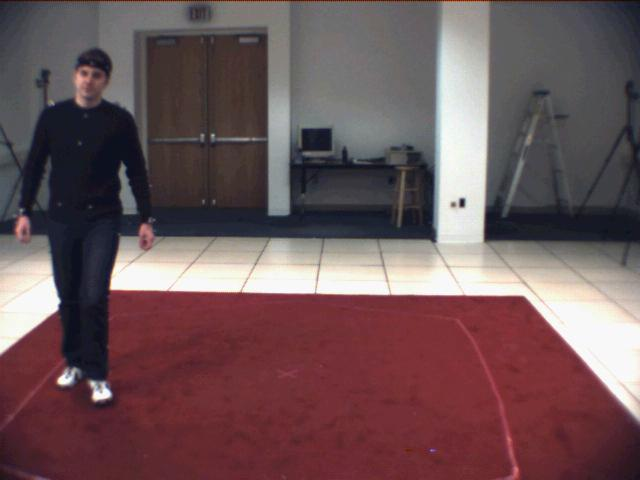
\includegraphics[height=5.5cm]{wrongimage}}
  \subcaptionbox{错误骨架}{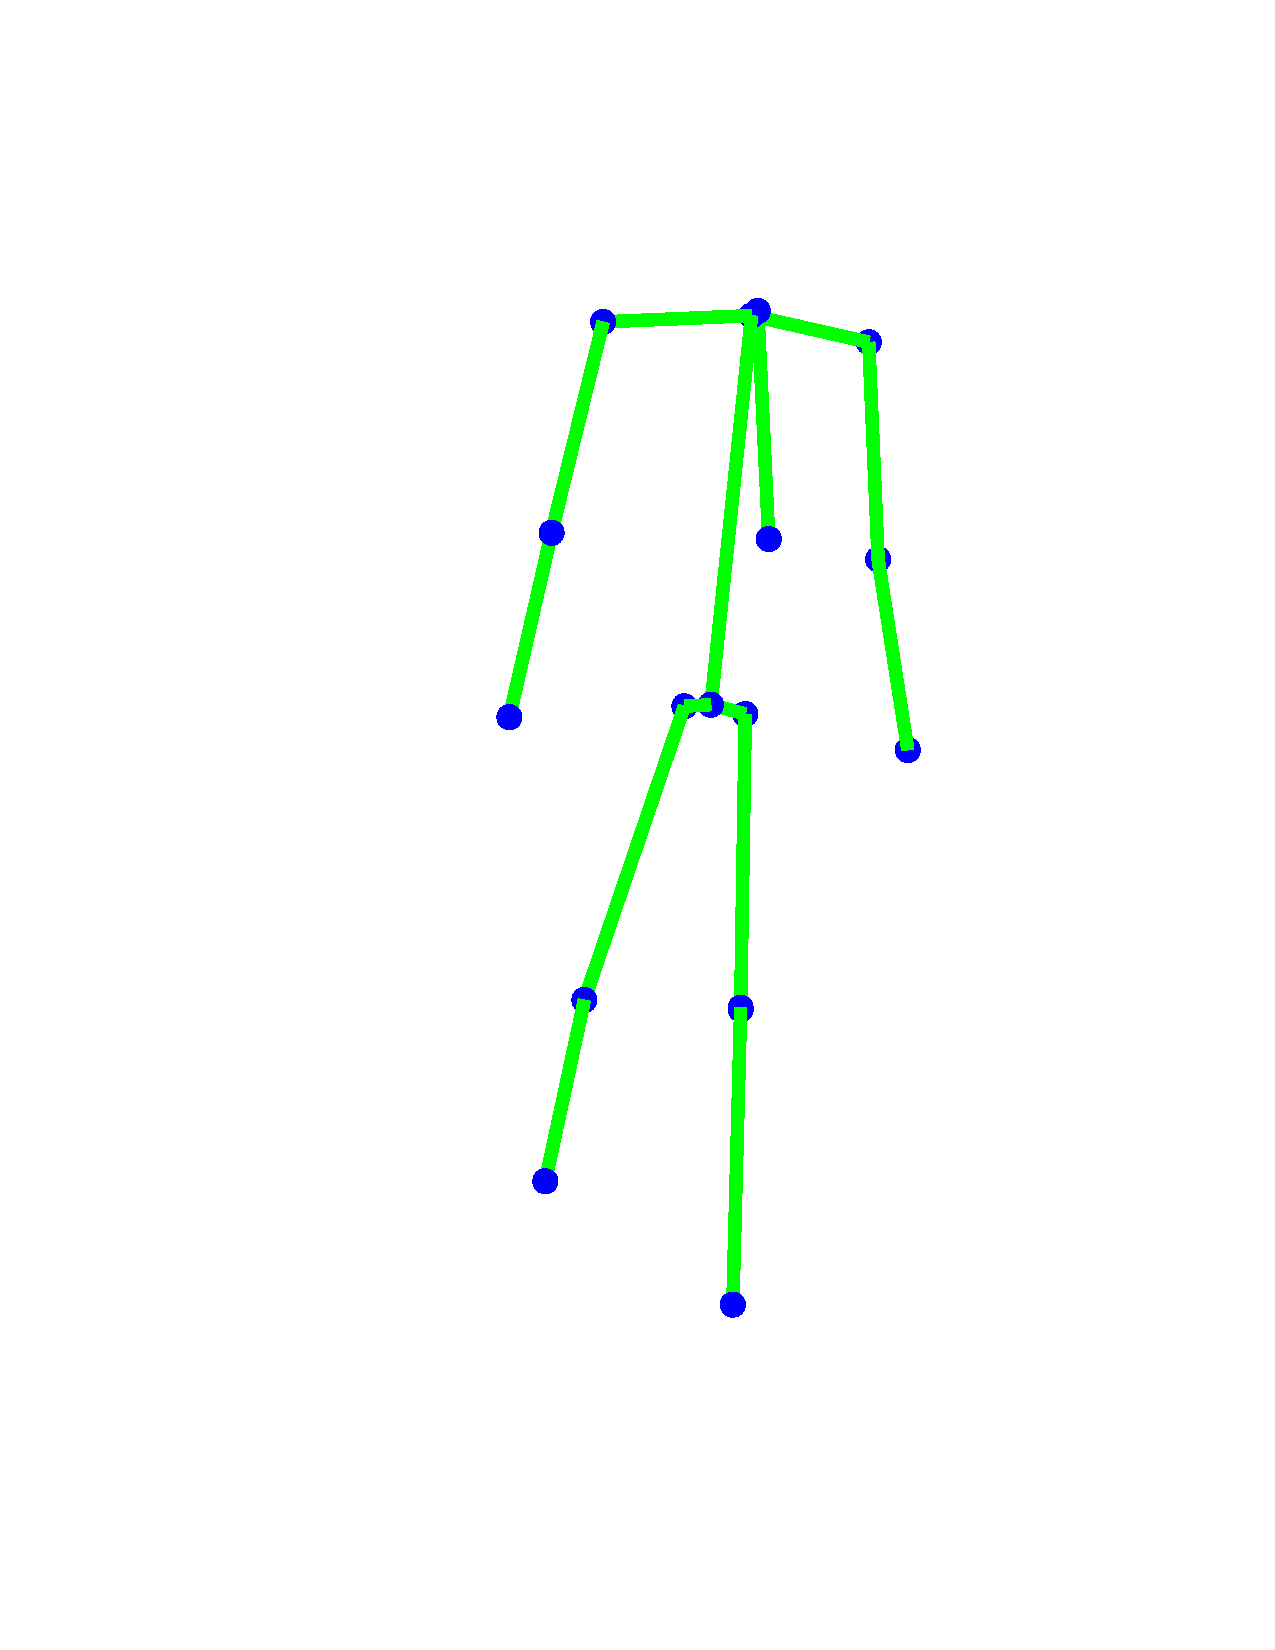
\includegraphics[height=5.5cm]{wrong}}
  \caption{错误的ground-truth}\label{fig:wrong}
\end{figure}

本文采用了不同的特征得到了较差的结果,说明了预测结果和特征关系极大,由于这次的实验十分耗时,我没能用更多的时间去选择合适的特征,我非常遗憾。在接下来的工作中,我希望能提出一种更有效的特征来解决这个问题。但是只去选择更合适的特征意义并不大,综合一些文献~\cite{ramanan2007learning}~\cite{yang2011articulated}的思路,我认为在解决人体姿态估计问题中需要分层处理,即先识别各个肢体的位置和姿态,然后再全局优化。用本文中所述将所有信息一起训练是冗余且低效的,即使用了多达10000帧的数据,并且动作简单到只有几类,效果仍然不是很好。只有好的特征配合高效的算法才能实现更好的预测结果。

\section{收获与体会}
首先,我认为选题是非常重要的环节。在毕业设计初期,我一直在做很多尝试,调查了很多方向,也阅读了相当多的文献,但都没有找到合适的方向下手。当考虑做多人体三维建模时发现难度很大,于是不断缩小目标,最后落脚到单人体三维姿态估计,即便如此,经过调查我发现这是一个由来已久的难题,于是只好摸索着前进。前期调研花掉了较多的时间,导致后期做实验的时间被大大缩短,也导致了结果的不理想。

其次,我体会到了做图像处理实验的难处。第一,数据库很重要,巧妇难为无米之炊,也正如文献~\cite{gkiox2013ariarticulated}所说那样:\\
\begin{center}
\shadowbox{
\begin{minipage}{8cm}
\thispagestyle{plain}
We give the last word to Sherlock Holmes:\\
“Data! Data! Data!” he cried impatiently. “I can't make bricks without clay.”\\
\emph{The Adventure of the Copper Beeches}
\end{minipage}}
\end{center}
没有数据就没办法实验,好在本文可以利用HumanEva数据库,在此十分感谢布朗大学。第二点难处是时间,做实验非常漫长,需要很好的耐心,不能轻易放弃。在我没有结果的时候,我的朋友给了我鼓励和帮助,让我坚持了下去,我很感激他们。

当然,我收获了很多知识,不仅仅是人体姿态识别这个领域我了解了最流行最有效的方法,我还在前期调研中探索了很多其他领域,比如图片拼接、3D视频质量评价、去模糊、三维重建、霍夫树等。收获的也不止是知识,还有学习的方法,熟悉了如何调研、查阅文献,怎么去网上找到可以利用的代码和数据库等等。